% !TeX root = writeup.tex 
\section{Simulations}

We examine the outcomes induced by fairness constraints in the context of FICO scores for two race groups. FICO scores are a proprietary classifier widely used in the United States to predict credit worthiness. Our FICO data is based on a sample of 301,536 TransUnion TransRisk scores from 2003 \citep{fed07}, preprocessed by \citet{hardt16equality}. These scores, corresponding to $x$ in our model, range from 300 to 850 and are meant to predict credit risk. Empirical data labeled by race allows us to estimate the distributions $\pi\supj$, where $\popj$ represents race, which is restricted to two values: white non-Hispanic (labeled ``white" in figures), and black. Using national demographic data, we set the population proportions to be $18\%$ and $82\%$.

Individuals were labeled as defaulted if they failed to pay a debt for at least 90 days on at least one account in the ensuing 18-24 month period; we use this data to estimate the success probability given score, $\pb\supj(x)$, which we allow to vary by group to match the empirical data (see Figure~\ref{fig:empirical_payback_probs}). Our outcome curve framework allows for this relaxation; however, this discrepancy can also be attributed to group-dependent mismeasurement of score, and adjusting the scores accordingly would allow for a single $\pb(x)$. We use the success probabilities to define the affine utility and score change functions defined in Example~\ref{ex:credit_lending}. We model individual penalties as a score drop of $c_-=-150$ in the case of a default, and in increase of $c_+=75$ in the case of successful repayment.

\begin{figure*}[t] %  figure placement: here, top, bottom, or page
   \centering
   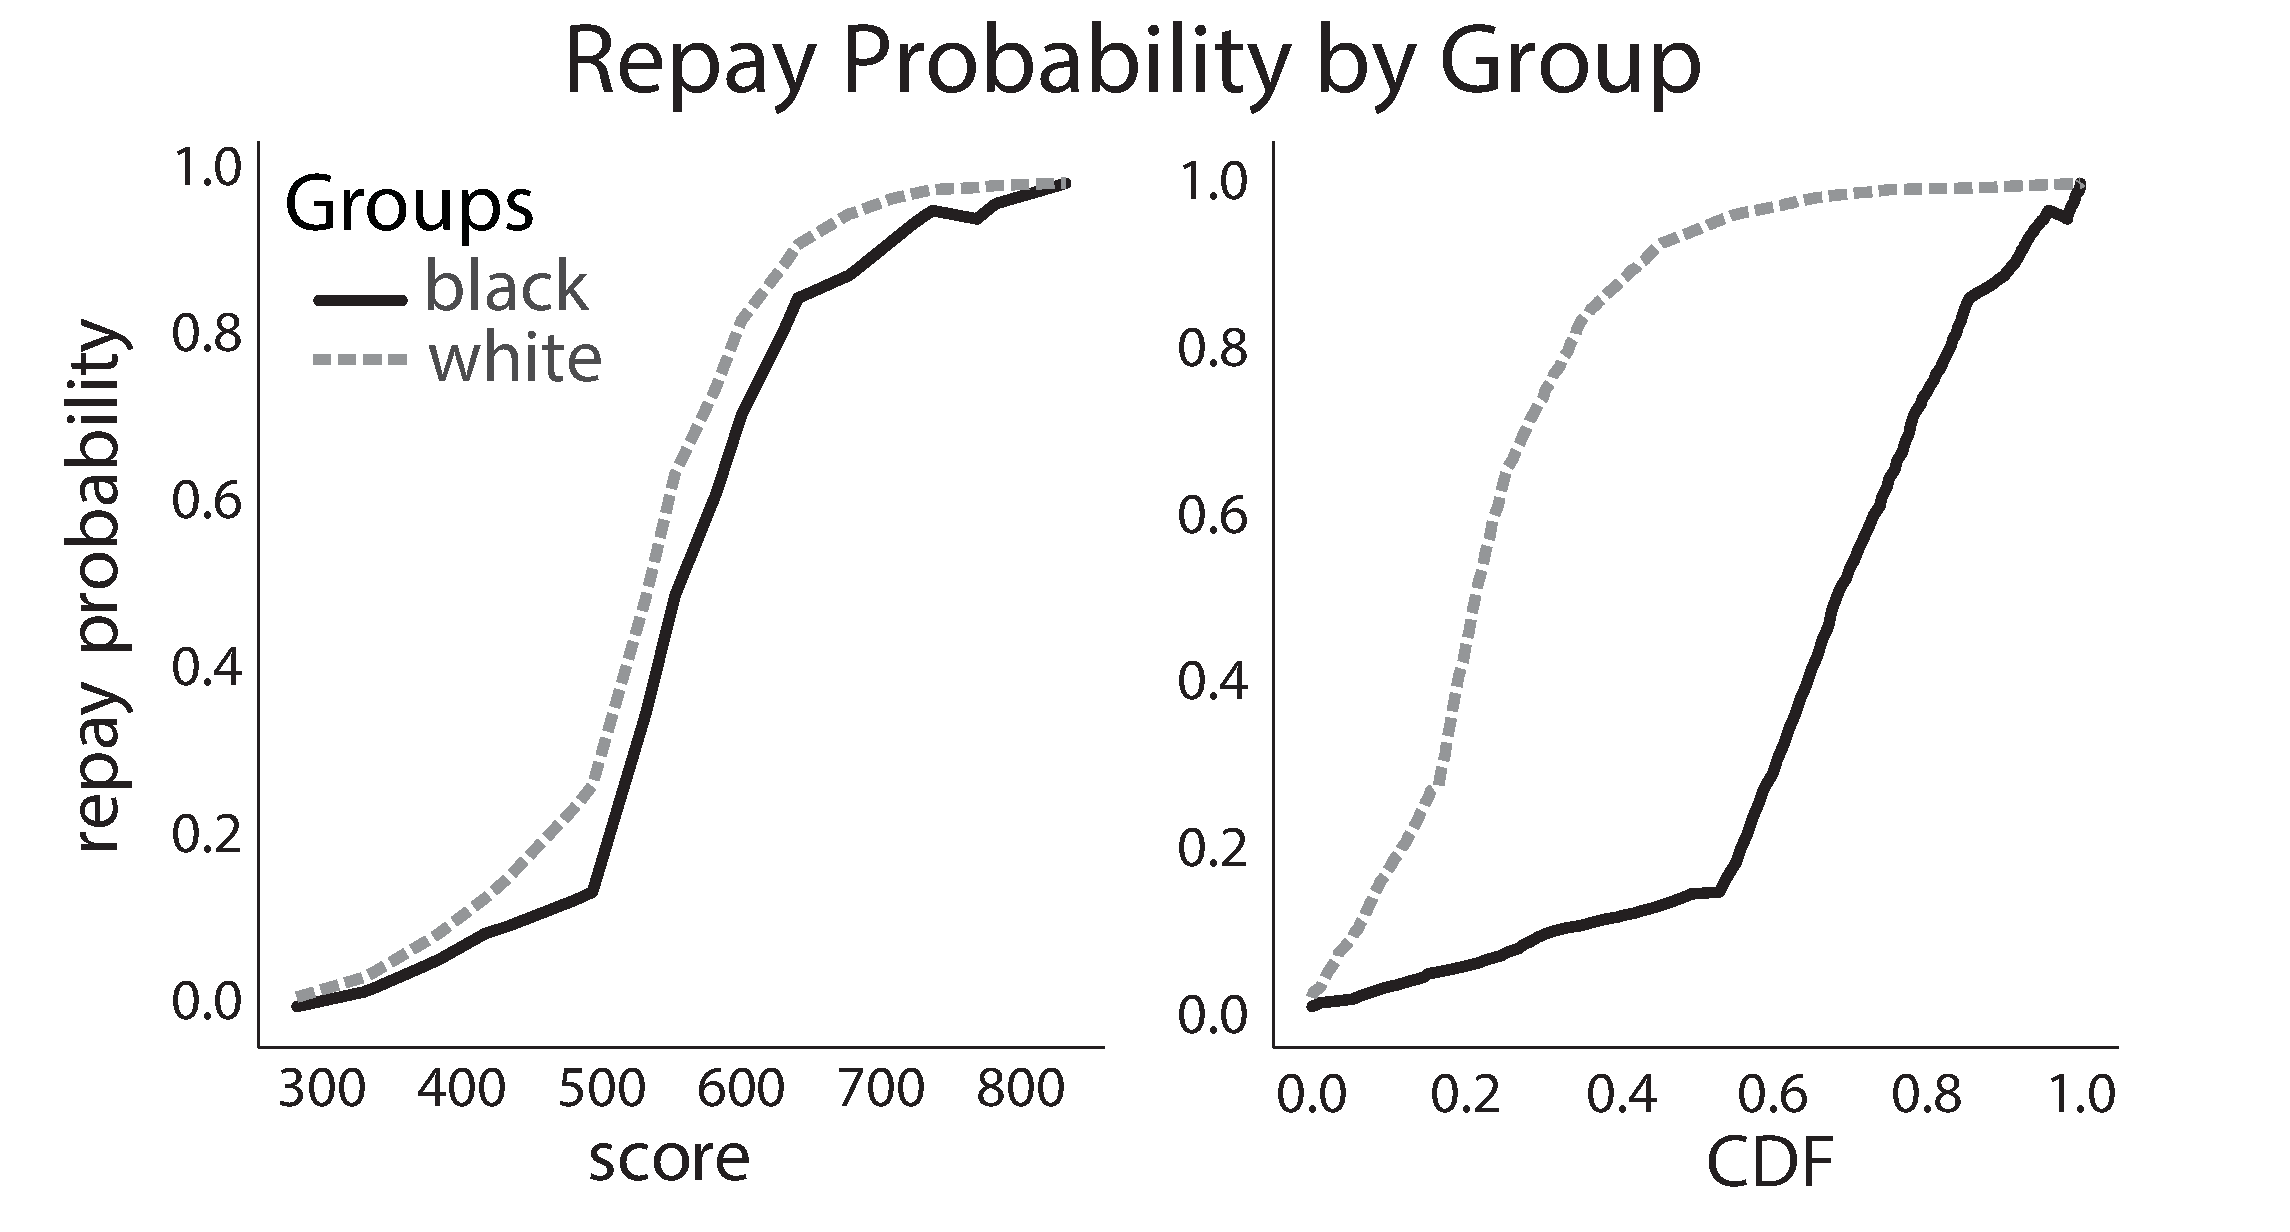
\includegraphics[width=0.7\textwidth]{figures/empirical_data/repay_probs.pdf}
   \caption{The empirical payback rates as a function of credit score and CDF for both groups from the TransUnion TransRisk dataset.}
   \label{fig:empirical_payback_probs}
\end{figure*}


\begin{figure*}[t] %  figure placement: here, top, bottom, or page
   \centering
   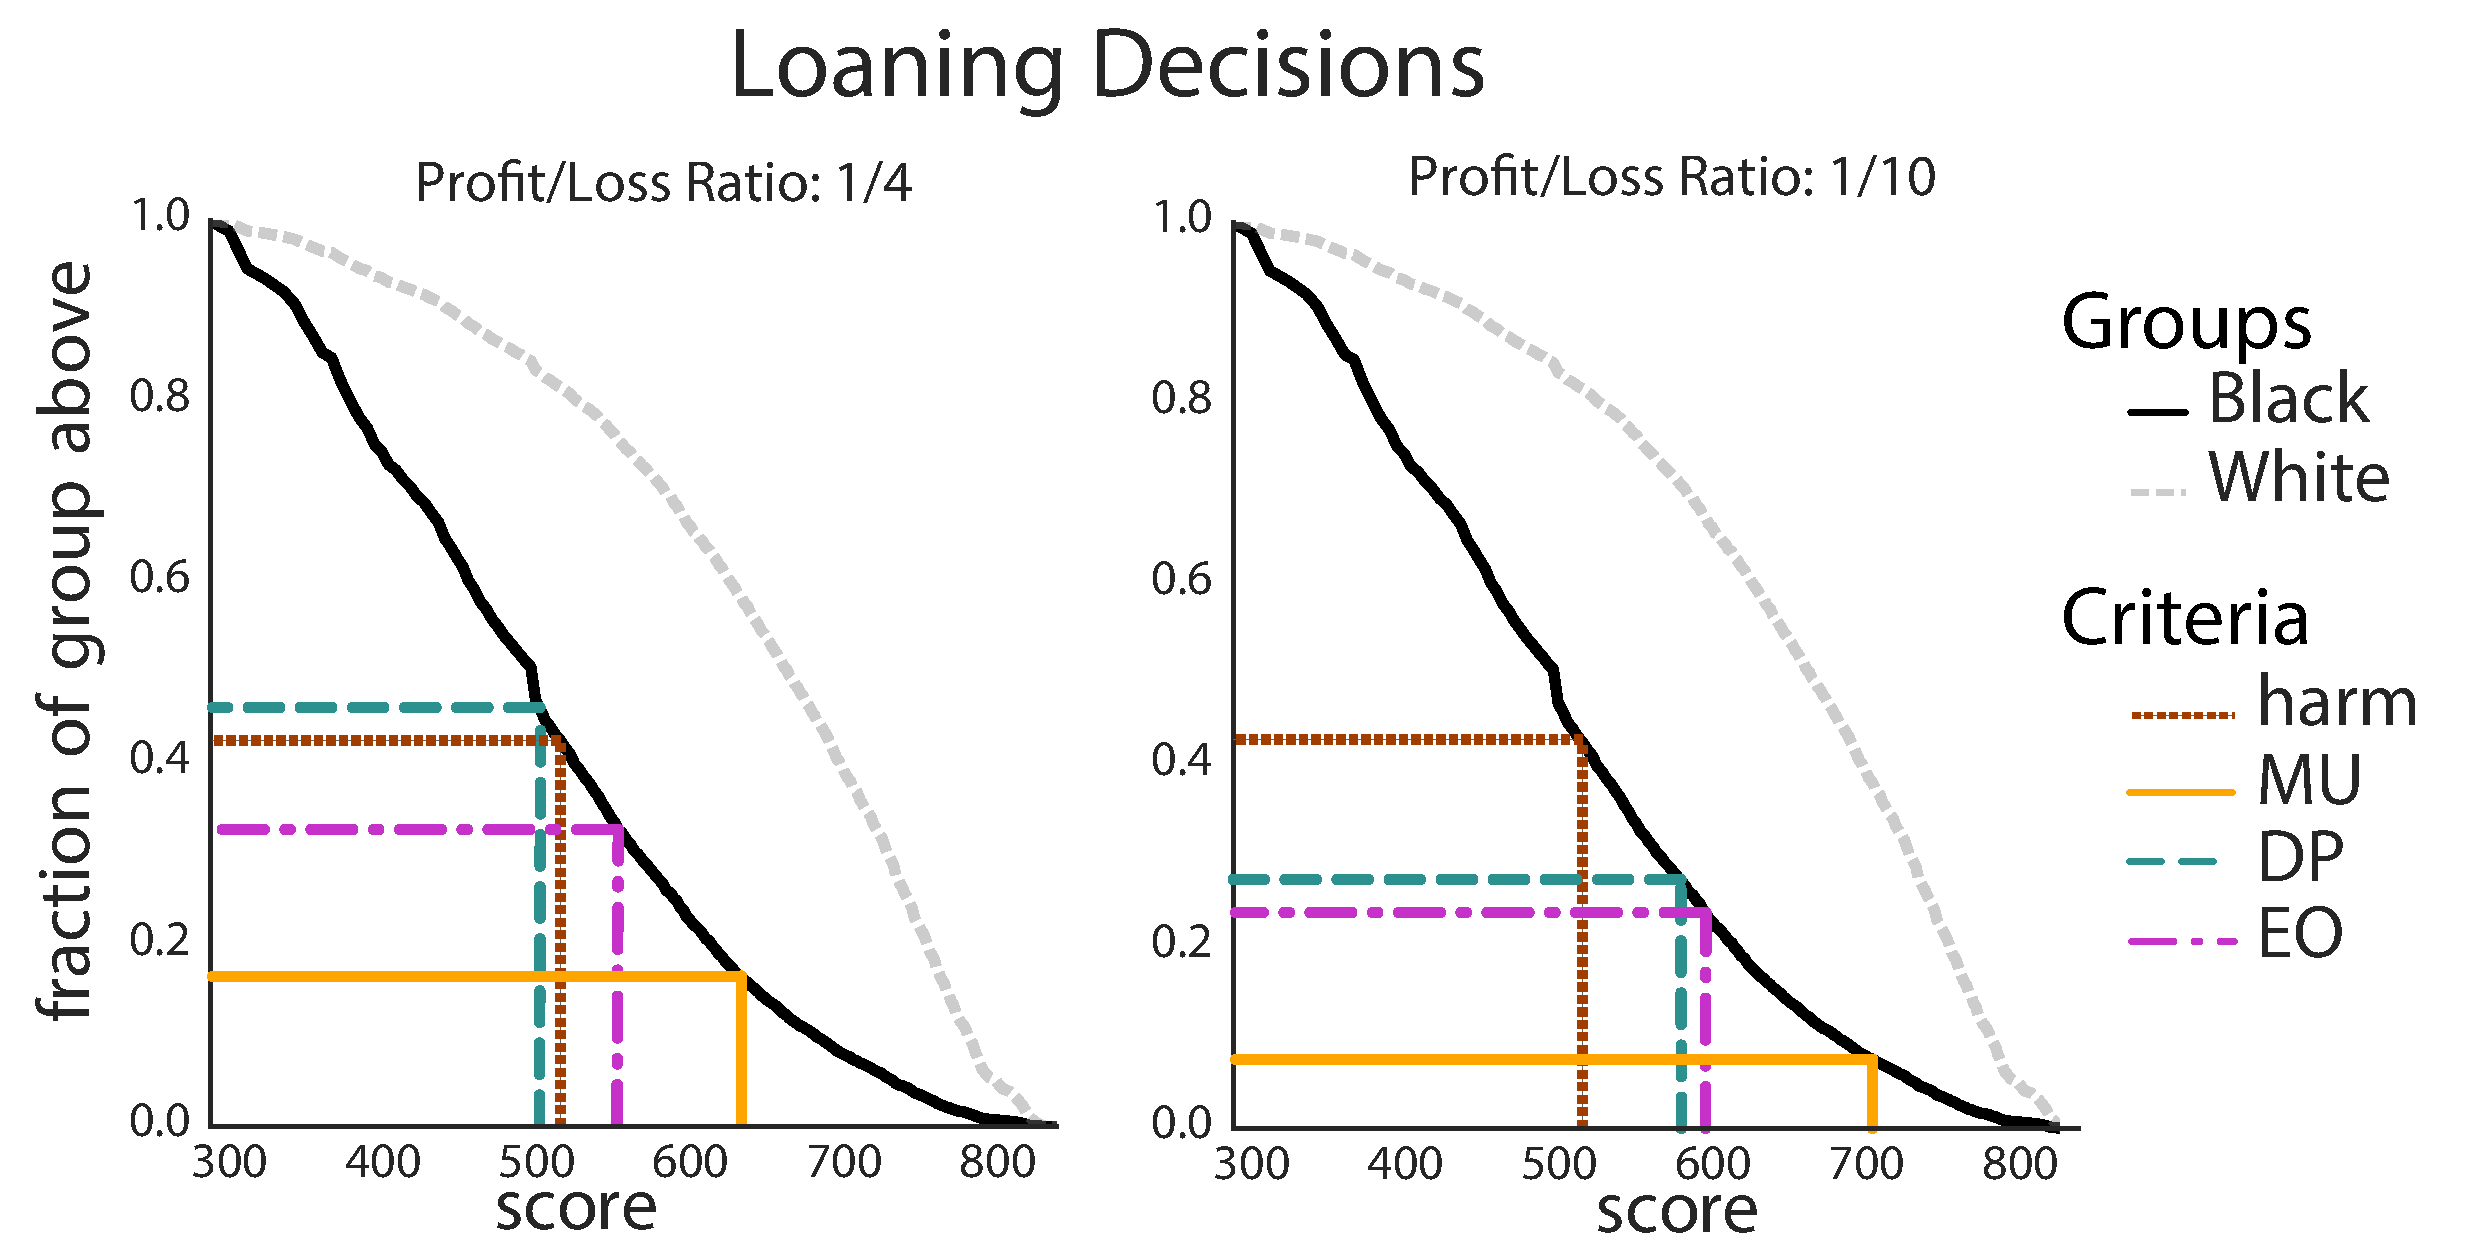
\includegraphics[width=0.7\textwidth]{figures/empirical_data/cdfs_both.pdf}
   \caption{The empirical CDFs of both groups are plotted along with the decision thresholds resulting from $\maxprof$, $\dempar$, and $\eqop$ for a model with bank utilities set to (a) $\frac{u_-}{u_+} = -4$ and (b) $\frac{u_-}{u_+} = -10$. The threshold for active harm is displayed; in (a) $\dempar$ causes active harm while in (b) it does not. $\eqop$ and $\maxprof$ never cause active harm.}
   \label{fig:empirical_outcome1}
\end{figure*}

In Figure~\ref{fig:empirical_outcome1}, we display the empirical CDFs along with selection rates resulting from different loaning strategies for two different settings of bank utilities. In the case that the bank experiences a loss/profit ratio of $\frac{u_-}{u_+} = -10$, no fairness criteria surpass the active harm rate $\accrate_0$; however, in the case of $\frac{u_-}{u_+} = -4$, $\dempar$ overloans, in line with the statement in Corollary~\ref{cor:dp_overeager}.

These results are further examined in Figure~\ref{fig:empirical_outcome}, which displays the normalized outcome curves and the utility curves for both the white and the black group. To plot the $\maxprof$ utility curves, the group that is not on display has selection rate fixed at $\beta^{\maxprof}$. In this figure, the top panel corresponds to the average change in credit scores for each group under different loaning rates $\accrate$; the bottom panels shows the corresponding \emph{total} utility $\Util$ (summed over both groups and weighted by group population sizes) for the bank. %Therefore, for the bottom group 

Figure~\ref{fig:empirical_outcome} highlights that the position of the utility optima in the lower panel determines the loan (selection) rates. In this specific instance, the utility and change ratios are fairly close, $\frac{u_-}{u_+} = -4$, and $\frac{c_-}{c_+} = -2$, meaning that the bank's profit motivations align with individual outcomes to some extent. Here, we can see that $\eqop$ loans much closer to optimal than $\dempar$, similar to the setting suggested by Corollary~\ref{cor:fairness_rel_imp}.

Although one might hope for decisions made under fairness constraints to positively affect the black group, we observe the opposite behavior. The $\maxprof$ policy (solid orange line) and the $\eqop$ policy result in similar expected credit score change for the black group. However, $\dempar$ (dashed green line) causes a negative expected credit score change in the black group, corresponding to active harm. For the white group, the bank utility curve has almost the same shape under the fairness criteria as it does under $\maxprof$, the main difference being that fairness criteria lowers the total expected profit from this group. 


This behavior stems from a discrepancy in the outcome and profit curves for each population. While incentives for the bank and positive results for individuals are somewhat aligned for the majority group, under fairness constraints, they are more heavily misaligned in the minority group, as seen in graphs (left) in Figure~\ref{fig:empirical_outcome}. We remark that in other settings where the \emph{unconstrained} profit maximization is misaligned with individual outcomes (e.g., when $\frac{u_-}{u_+} = -10$), fairness criteria may perform more favorably for the minority group by pulling the utility curve into a shape consistent with the outcome curve.

By analyzing the resulting affects of $\maxprof$, $\dempar$, and $\eqop$ on actual credit score lending data, we show the applicability of our model to real-world applications. In particular, some results shown in Section~\ref{sec:results} hold empirically for the FICO TransUnion TransRisk scores.


\begin{figure}[p] %  figure placement: here, top, bottom, or page
	\centering
	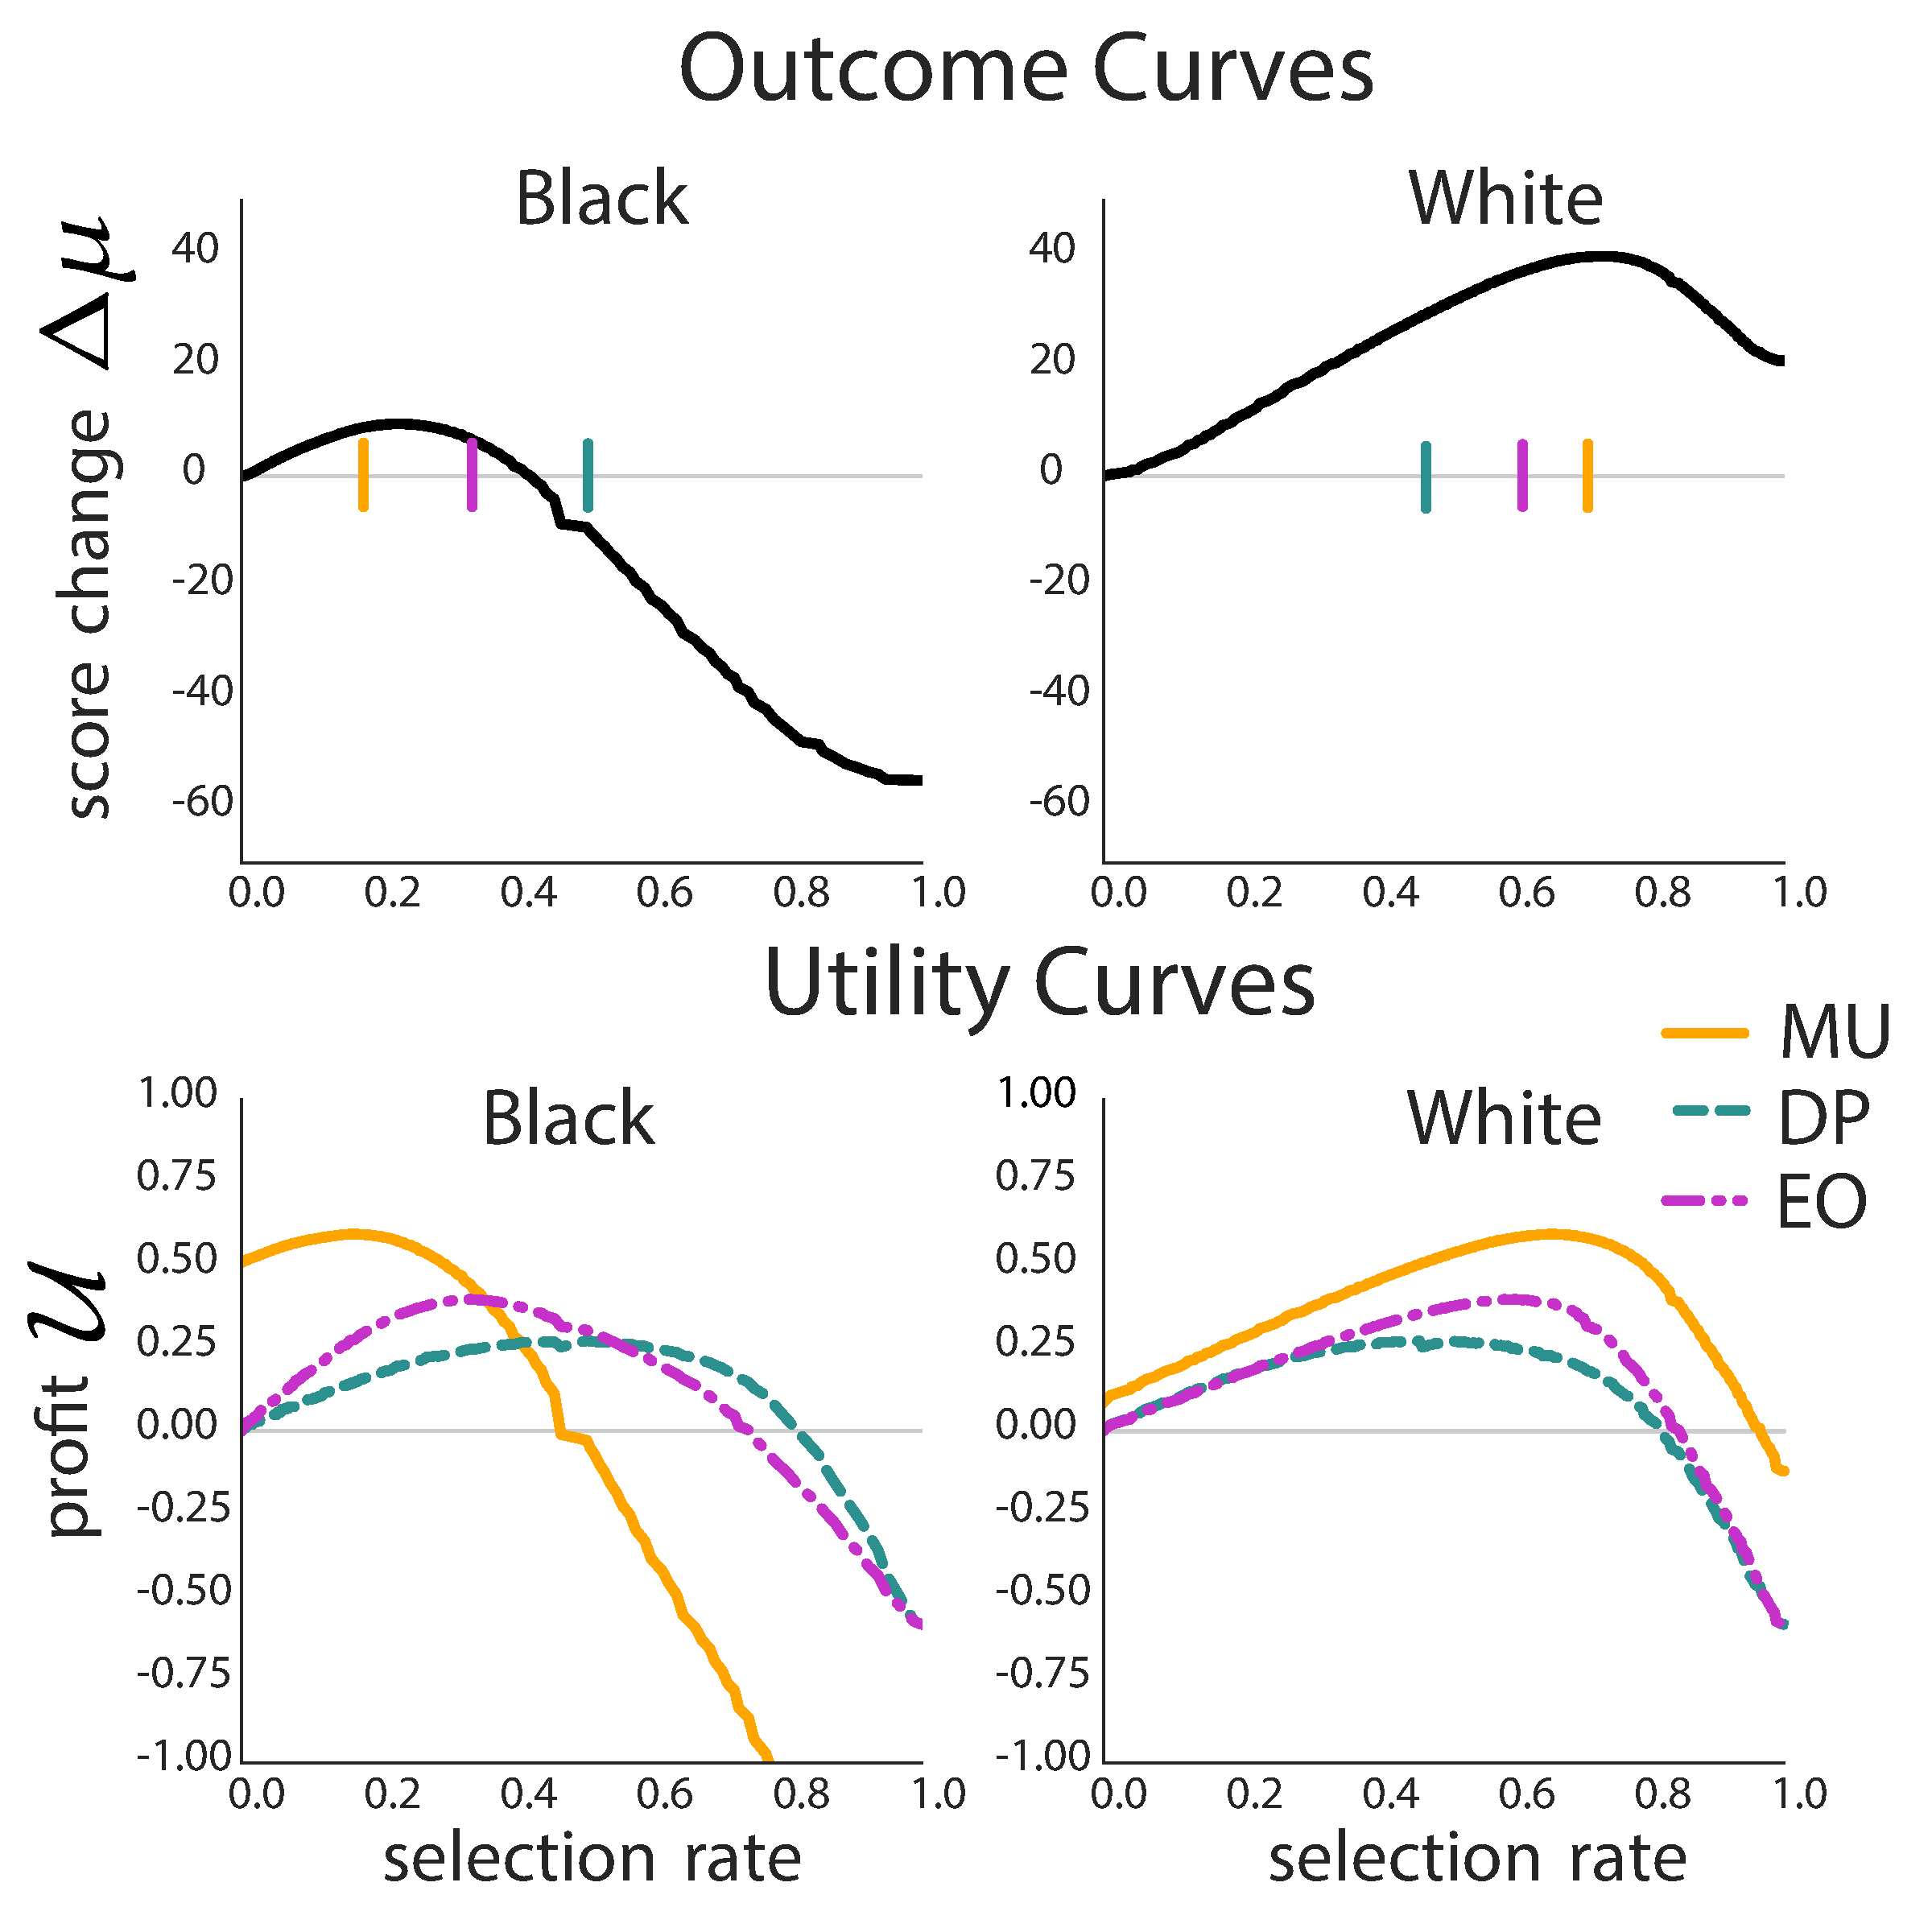
\includegraphics[width=.9\columnwidth]{figures/empirical_data/emp_outcome_curves.pdf}
	\caption{The outcome and utility curves are plotted for both groups against the group selection rates. The relative positions of the utility maxima determine the position of the decision rule thresholds. We hold $\frac{u_-}{u_+} = -4$ as fixed. %Note that t we can see that the advantage of the white group cases $\dempar$ to cause active harm for the black group. 
	}
	\label{fig:empirical_outcome}
\end{figure}




